%% LaTeX-Beamer template for KIT design
%% by Erik Burger, Christian Hammer
%% title picture by Klaus Krogmann
%%
%% version 2.1
%%
%% mostly compatible to KIT corporate design v2.0
%% http://intranet.kit.edu/gestaltungsrichtlinien.php
%%
%% Problems, bugs and comments to
%% burger@kit.edu

\documentclass[18pt]{beamer}

%% SLIDE FORMAT

% use 'beamerthemekit' for standard 4:3 ratio
% for widescreen slides (16:9), use 'beamerthemekitwide'

\usepackage{templates/beamerthemekit}
% \usepackage{templates/beamerthemekitwide}

\usepackage[utf8]{inputenc}
\usepackage{hyperref}
\usepackage{listings}
\usepackage{color}
\usepackage{xcolor}
\usepackage{colortbl}
\usepackage{array}
%\usepackage{tikz}
%\usetikzlibrary{calc,shapes.multipart,chains,arrows}
\usepackage{amsmath}
\usepackage{amssymb}
\usepackage{mathrsfs}

\definecolor{lime}{HTML}{8FFF53}
\definecolor{darkgrey}{HTML}{5A5A5A}
\definecolor{awesome}{HTML}{FF2252}
\definecolor{lightgreen}{HTML}{E0FF98}

\newcommand{\quotes}[1]{``#1''}

%% TITLE PICTURE

% if a custom picture is to be used on the title page, copy it into the 'logos'
% directory, in the line below, replace 'mypicture' with the
% filename (without extension) and uncomment the following line
% (picture proportions: 63 : 20 for standard, 169 : 40 for wide
% *.eps format if you use latex+dvips+ps2pdf,
% *.jpg/*.png/*.pdf if you use pdflatex)

\titleimage{greendrop}

%% TITLE LOGO

% for a custom logo on the front page, copy your file into the 'logos'
% directory, insert the filename in the line below and uncomment it

%\titlelogo{mylogo}

% (*.eps format if you use latex+dvips+ps2pdf,
% *.jpg/*.png/*.pdf if you use pdflatex)

%% TikZ INTEGRATION

% use these packages for PCM symbols and UML classes
% \usepackage{templates/tikzkit}
% \usepackage{templates/tikzuml}

% the presentation starts here

\title[Suchen, Sortieren, Parsen]{Programmieren:\\ Suchen, Sortieren, Parsen}
\subtitle{Tutorium 30}
\author{YouniS Bensalah}
\date{January 22, 2016}

\institute{Chair for Software Design and Quality}

% Bibliography

\usepackage[citestyle=authoryear,bibstyle=numeric,hyperref,backend=biber]{biblatex}
\addbibresource{templates/example.bib}
\bibhang1em

\begin{document}

% change the following line to "ngerman" for German style date and logos
\selectlanguage{english}

%title page
\begin{frame}
\titlepage
\end{frame}

%table of contents
\begin{frame}{Heute}
\tableofcontents
\end{frame}

\section{Organisatorisches}

\begin{frame}{Organisatorisches}
    \begin{itemize}
        \item Bewertung Programmieren
        \begin{itemize}
            \item Der Übungsschein muss bestanden werden, um zu den Abschlussaufgaben zugelassen zu werden.
            \item Der Übungsschein geht jedoch \textbf{nicht} in die Note mit ein.
            \item Die Note wird einzig durch das Abschneiden in den Abschlussaufgaben gebildet.
        \end{itemize}
        \vspace{.3in}
        \item Anmeldung Übungsschein und Abschlussaufgabe
        \begin{itemize}
            \item Es kann sein, dass es damit zurzeit Probleme gibt.
            \item \textit{Keep calm and retry later.}
        \end{itemize}
    \end{itemize}
\end{frame}

\section{Suchen}

\begin{frame}{Suchen}
    \center
    \Huge{Suchen}
\end{frame}

\begin{frame}{Suchen}
    \begin{block}{}
        \textbf{Problem:}\\
        \textit{\quotes{Wie finde ich ein bestimmtes Element in einer Liste ?}}
    \end{block}
    \vspace{.2in}
    \begin{center}
        \begin{tabular}{|c|c|c|c|c|c|c|c|}
            \hline
            4 & 2 & 3 & 9 & 7 & 13 & 6 & 10 \\
            \hline
        \end{tabular}
    \end{center}
\end{frame}

\subsection{Lineare Suche}

\begin{frame}{Lineare Suche}
    \begin{itemize}
        \item Erster (naiver) Ansatz: \textbf{Lineare Suche}
        \item Idee: Ein Element nach dem anderen anschauen und vergleichen.
    \end{itemize}
\end{frame}

\begin{frame}[fragile]{Lineare Suche: Java-Code}
    \begin{exampleblock}{}
        \begin{lstlisting}[language=Java,basicstyle=\scriptsize]
int linearSearch(int needle, int[] haystack) {
    for (int i = 0; i < haystack.length; i++) {
        if (haystack[i] == needle) {
            return i;
        }
    }
    return -1;
}
        \end{lstlisting}

    \end{exampleblock}

\end{frame}

\begin{frame}{Lineare Suche}
    \begin{itemize}
        \item Laufzeit: $\mathcal{O}(n)$
        \item Für beliebige Listen geht es nicht wirklich besser.
    \end{itemize}
\end{frame}

\subsection{Binäre Suche}

\begin{frame}{Rätsel}
    \small
    Es wurde ein neuer Info-Bau an der Uni errichtet. Das neue Gebäude besitzt ganze 256 Stockwerke.
    Die Informatiker sind zunächst begeistert, doch schon bald gibt es ein Problem:\\
    Da bekanntlich alle Informatiker Keller gewohnt sind, können sie die Gefahr von offenen Fenstern nicht einschätzen und fallen gelegentlich hinaus.\\
    Daraufhin sollten zunächst alle Fenster des Gebäudes verriegeln werden, doch man hat festgestellt, dass einige Informatiker den Sturz munter überstanden haben.\\
    Nun geht man davon aus, dass es ein Stockwerk $n$ gibt, ab dem die Fenster keine Gefahr mehr darstellen. Zu diesem Zweck sollen nun Tests durchgeführt werden,
    bei denen man jeweils einen Informatiker aus dem Fenster springen lässt und beobachtet, ob der Sturz munter überstanden wurde.
    Da die Informatiker aber lieber die Anzahl der Tests als die Anzahl der unglücklichen Landungen minimieren wollen, kommt eine lineare Suche (Stockwert 1, Stockwerk 2, \dots) nicht in Frage.\\
    \vspace{.2in}
    Wieviele \quotes{Testfälle} braucht man im ungünstigsten Fall ?
\end{frame}

\begin{frame}{Lösung}
    \begin{block}{}
        $log_2(256) = log_2(2^8) = 8$
    \end{block}
    \pause
    \vspace{.4in}
    \textit{\dots Aber warum ?}
\end{frame}


\begin{frame}{Binäre Suche}
    \begin{itemize}
        \item Ansatz: Suche auf einer vorsortierten Liste.
        \item Idee: Teile die Liste in zwei Hälften und entscheide, in welcher der beiden Teillisten das gesuchte Element liegt und verwerfe die andere.\\
        Dann wiederhole den Vorgang auf der übrigen Liste.
    \end{itemize}
\end{frame}

\begin{frame}[fragile]{Binäre Suche: Java-Code}
    \begin{exampleblock}{}
        \begin{lstlisting}[language=Java,basicstyle=\scriptsize]
int binarySearch(int needle, int[] haystack, int from, int to) {
    if (to > from) {
        int mid = (from + to) / 2;
        if (needle < haystack[mid]) {
            return search(needle, haystack, from, mid - 1);
        } else if (needle > haystack[mid]) {
            return search(needle, haystack, mid + 1, to);
        } else {
            return mid;
        }
    }
    return -1;
}
        \end{lstlisting}
    \end{exampleblock}
\end{frame}

\begin{frame}{Binäre Suche: Beispiel}
    Suche: \textbf{\alert{8}}
    \begin{center}
        \begin{tabular}{|c|c|c|c|c|c|c|c|c|c|c|c|c|c|c|c|}
            \hline
            \cellcolor{lightgreen}{3} & \cellcolor{lightgreen}{4} & \cellcolor{lightgreen}{4} & \cellcolor{lightgreen}{5} & \cellcolor{lightgreen}{6} & \cellcolor{lightgreen}{7} & \cellcolor{lightgreen}{8} & \cellcolor{lightgreen}{10} & \cellcolor{lightgreen}{11} & \cellcolor{lightgreen}{14} & \cellcolor{lightgreen}{17} & \cellcolor{lightgreen}{22} & \cellcolor{lightgreen}{24} & \cellcolor{lightgreen}{29} & \cellcolor{lightgreen}{32} & \cellcolor{lightgreen}{42} \\
            \hline
        \end{tabular}
        \pause
        \begin{tabular}{|c|c|c|c|c|c|c|c|c|c|c|c|c|c|c|c|}
            \hline
            \cellcolor{lightgreen}{3} & \cellcolor{lightgreen}{4} & \cellcolor{lightgreen}{4} & \cellcolor{lightgreen}{5} & \cellcolor{lightgreen}{6} & \cellcolor{lightgreen}{7} & \cellcolor{lightgreen}{8} & \cellcolor{lightgreen}{10} & \cellcolor{lime}{11} & \cellcolor{darkgrey}{14} & \cellcolor{darkgrey}{17} & \cellcolor{darkgrey}{22} & \cellcolor{darkgrey}{24} & \cellcolor{darkgrey}{29} & \cellcolor{darkgrey}{32} & \cellcolor{darkgrey}{42} \\
            \hline
        \end{tabular}
        \pause
        \begin{tabular}{|c|c|c|c|c|c|c|c|c|c|c|c|c|c|c|c|}
            \hline
            \cellcolor{darkgrey}{3} & \cellcolor{darkgrey}{4} & \cellcolor{darkgrey}{4} & \cellcolor{lime}{5} & \cellcolor{lightgreen}{6} & \cellcolor{lightgreen}{7} & \cellcolor{lightgreen}{8} & \cellcolor{lightgreen}{10} & \cellcolor{darkgrey}{11} & \cellcolor{darkgrey}{14} & \cellcolor{darkgrey}{17} & \cellcolor{darkgrey}{22} & \cellcolor{darkgrey}{24} & \cellcolor{darkgrey}{29} & \cellcolor{darkgrey}{32} & \cellcolor{darkgrey}{42} \\
            \hline
        \end{tabular}
        \pause
        \begin{tabular}{|c|c|c|c|c|c|c|c|c|c|c|c|c|c|c|c|}
            \hline
            \cellcolor{darkgrey}{3} & \cellcolor{darkgrey}{4} & \cellcolor{darkgrey}{4} & \cellcolor{darkgrey}{5} & \cellcolor{darkgrey}{6} & \cellcolor{lime}{7} & \cellcolor{lightgreen}{8} & \cellcolor{lightgreen}{10} & \cellcolor{darkgrey}{11} & \cellcolor{darkgrey}{14} & \cellcolor{darkgrey}{17} & \cellcolor{darkgrey}{22} & \cellcolor{darkgrey}{24} & \cellcolor{darkgrey}{29} & \cellcolor{darkgrey}{32} & \cellcolor{darkgrey}{42} \\
            \hline
        \end{tabular}
        \pause
        \begin{tabular}{|c|c|c|c|c|c|c|c|c|c|c|c|c|c|c|c|}
            \hline
            \cellcolor{darkgrey}{3} & \cellcolor{darkgrey}{4} & \cellcolor{darkgrey}{4} & \cellcolor{darkgrey}{5} & \cellcolor{darkgrey}{6} & \cellcolor{darkgrey}{7} & \cellcolor{lime}{8} & \cellcolor{lightgreen}{10} & \cellcolor{darkgrey}{11} & \cellcolor{darkgrey}{14} & \cellcolor{darkgrey}{17} & \cellcolor{darkgrey}{22} & \cellcolor{darkgrey}{24} & \cellcolor{darkgrey}{29} & \cellcolor{darkgrey}{32} & \cellcolor{darkgrey}{42} \\
            \hline
        \end{tabular}
        \pause
        \begin{tabular}{|c|c|c|c|c|c|c|c|c|c|c|c|c|c|c|c|}
            \hline
            \cellcolor{darkgrey}{3} & \cellcolor{darkgrey}{4} & \cellcolor{darkgrey}{4} & \cellcolor{darkgrey}{5} & \cellcolor{darkgrey}{6} & \cellcolor{darkgrey}{7} & \cellcolor{awesome}{8} & \cellcolor{darkgrey}{10} & \cellcolor{darkgrey}{11} & \cellcolor{darkgrey}{14} & \cellcolor{darkgrey}{17} & \cellcolor{darkgrey}{22} & \cellcolor{darkgrey}{24} & \cellcolor{darkgrey}{29} & \cellcolor{darkgrey}{32} & \cellcolor{darkgrey}{42} \\
            \hline
        \end{tabular}
    \end{center}
\end{frame}


\begin{frame}{Binäre Suche}
    \begin{itemize}
        \item Laufzeit: $\mathcal{O}(log(n))$
        \item Die Liste muss \textbf{sortiert} sein.
    \end{itemize}
\end{frame}

\section{Sortieren}

\begin{frame}{Sortieren}
    \center
    \Huge{Sortieren}
\end{frame}

\begin{frame}{Sortieren}
    \begin{block}{}
        \textbf{Problem:}\\
        \textit{\quotes{Wie sortiere ich eine gegebene Liste ?}}
    \end{block}
    \vspace{.2in}
    \begin{center}
        \begin{tabular}{|c|c|c|c|c|c|c|c|}
            \hline
            4 & 2 & 3 & 9 & 7 & 13 & 6 & 10 \\
            \hline
        \end{tabular}
    \end{center}
\end{frame}

\subsection{Bubble Sort}

\begin{frame}{Bubble Sort}
    \begin{itemize}
        \item Ansatz: Vertausche zwei unsortierte benachbarte Elemente, solange bis die Liste sortiert ist.
    \end{itemize}
    \vspace{.2in}
    \begin{figure}
        
\includegraphics[scale=.5]{img/BubbleSort.jpg}
    \end{figure}
\end{frame}

\begin{frame}[fragile]{Bubble Sort: Java-Code}
    \begin{exampleblock}{}
        \begin{lstlisting}[language=Java,basicstyle=\scriptsize]
void bubbleSort(int[] list) {
    int swap;
    for (int i = 1; i < list.length; i++) {
        for (int j = i; j > 0; j--) {
            if (list[j] < list[j - 1]) {
                swap = list[j];
                list[j] = list[j - 1];
                list[j - 1] = swap;
            }
        }
    }
}
        \end{lstlisting}
    \end{exampleblock}
\end{frame}

\subsection{Selection Sort}

\begin{frame}{Selection Sort}
    body
\end{frame}

\subsection{Insertion Sort}

\begin{frame}{Insertion Sort}
    body
\end{frame}

\subsection{Merge Sort}

\begin{frame}{Merge Sort}
    body
\end{frame}

\section{Parsen}

\begin{frame}{Parsen}
    \center
    \Huge{Parsen}
\end{frame}

\begin{frame}{Parsen}
    body
\end{frame}

\subsection{Formale Grammatiken}

\begin{frame}{Formale Grammatiken}
    body
\end{frame}

\subsection{Top-down Parsing}

\begin{frame}{Top-down Parsing}
    body
\end{frame}

\subsubsection{LL(1)-Parser}

\begin{frame}{LL(1)-Parser}
    body
\end{frame}

\appendix
\beginbackup

\begin{frame}{Fragen ?}
    \begin{figure}
        
\includegraphics[scale=.5]{img/formulas.png}
    \end{figure}
\end{frame}

\begin{frame}{Stack Sort}
    \url{https://gkoberger.github.io/stacksort}
\end{frame}

\begin{frame}{Bis nächste Woche !}
    \begin{figure}
        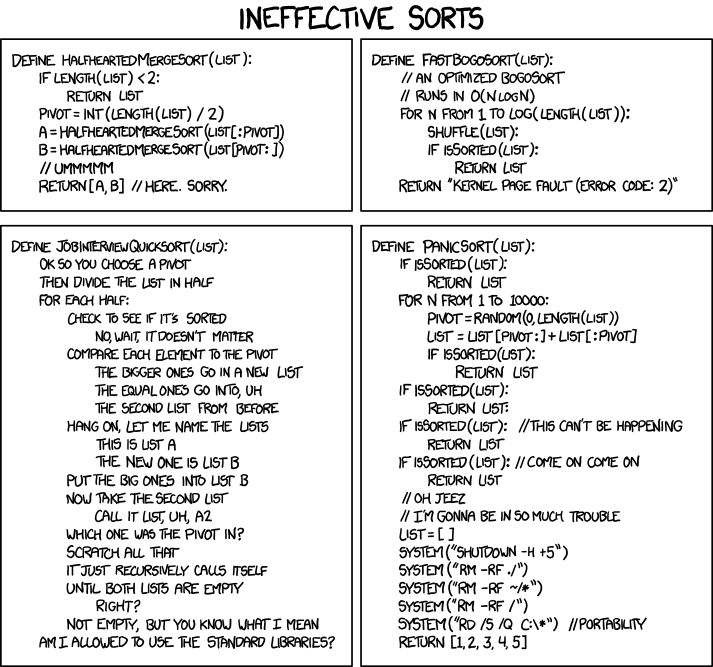
\includegraphics[scale=.3]{img/ineffective_sorts.png}
    \end{figure}
\end{frame}

\backupend

\end{document}
